\subsection{Beta version}
\label{kap:McpExecutorBetaversion}
Für die Betaversion der Mcp-Executor-Einheit werden alle Komponenten in ein Gehäuse integriert (s. Abbildung \ref{fig:McpExecutorBeta}), welches gerade so groß ist, dass es beim Tragen am Körper möglichst nicht stört und einfach befestigt werden kann. Für das Integrieren werden zusätliche Platinen angefertigt.
\newline
Aufgrund des Feststellens verschiedener negativer Aspekte während der Entstehung der EInheiten existieren mehrere Beta-Versionen.

\begin{enumerate}
	\item \textbf{Erste Beta-Version} \\
\begin{figure}[H]
	\centering
	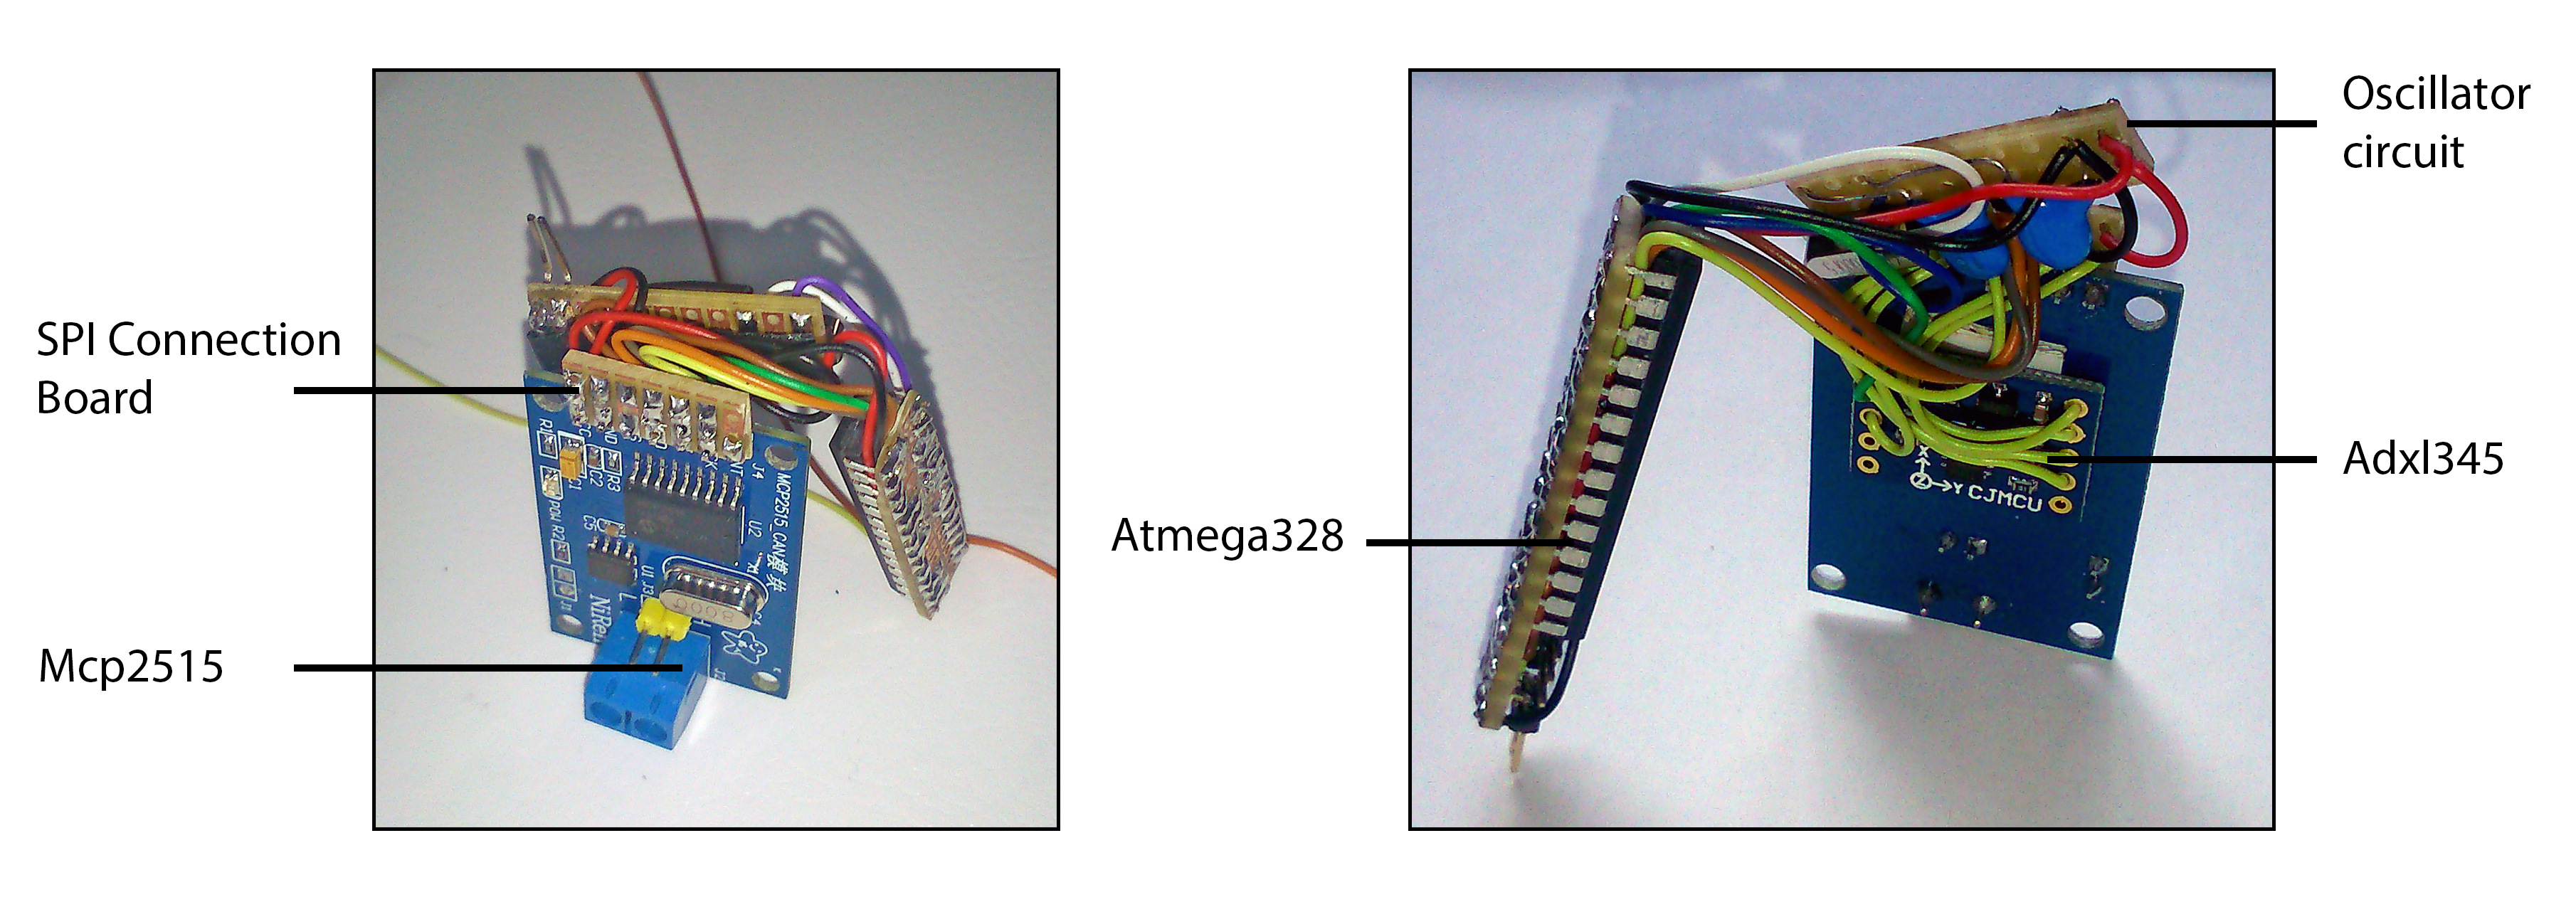
\includegraphics[width=1.0\linewidth]{Bilder/McpExecutor_BetaDetail}
	\caption[Betaversion einer Mcp-Executor-Einheit]{Betaversion einer Mcp-Executor-Einheit}
	\label{fig:McpExecutorBeta}
\end{figure}

Die Befestigung der Einheit am Körper erfolgt anhand eines Positioniergurtes. Dieser besteht in der ersten Beta-Version aus zwei und in der zweiten Version aus einem Klettverschluss, die an dem Abdeckblech der Einheit befestigt sind. Durch ein entsprechendes Gegenstück des Klettverschlusses auf der Rückseite des Abdeckblechs ist der notwendig Halt gegeben.
%
% BILD KLETTVERSCHLUSS
%
\begin{figure}[H]
	\centering
	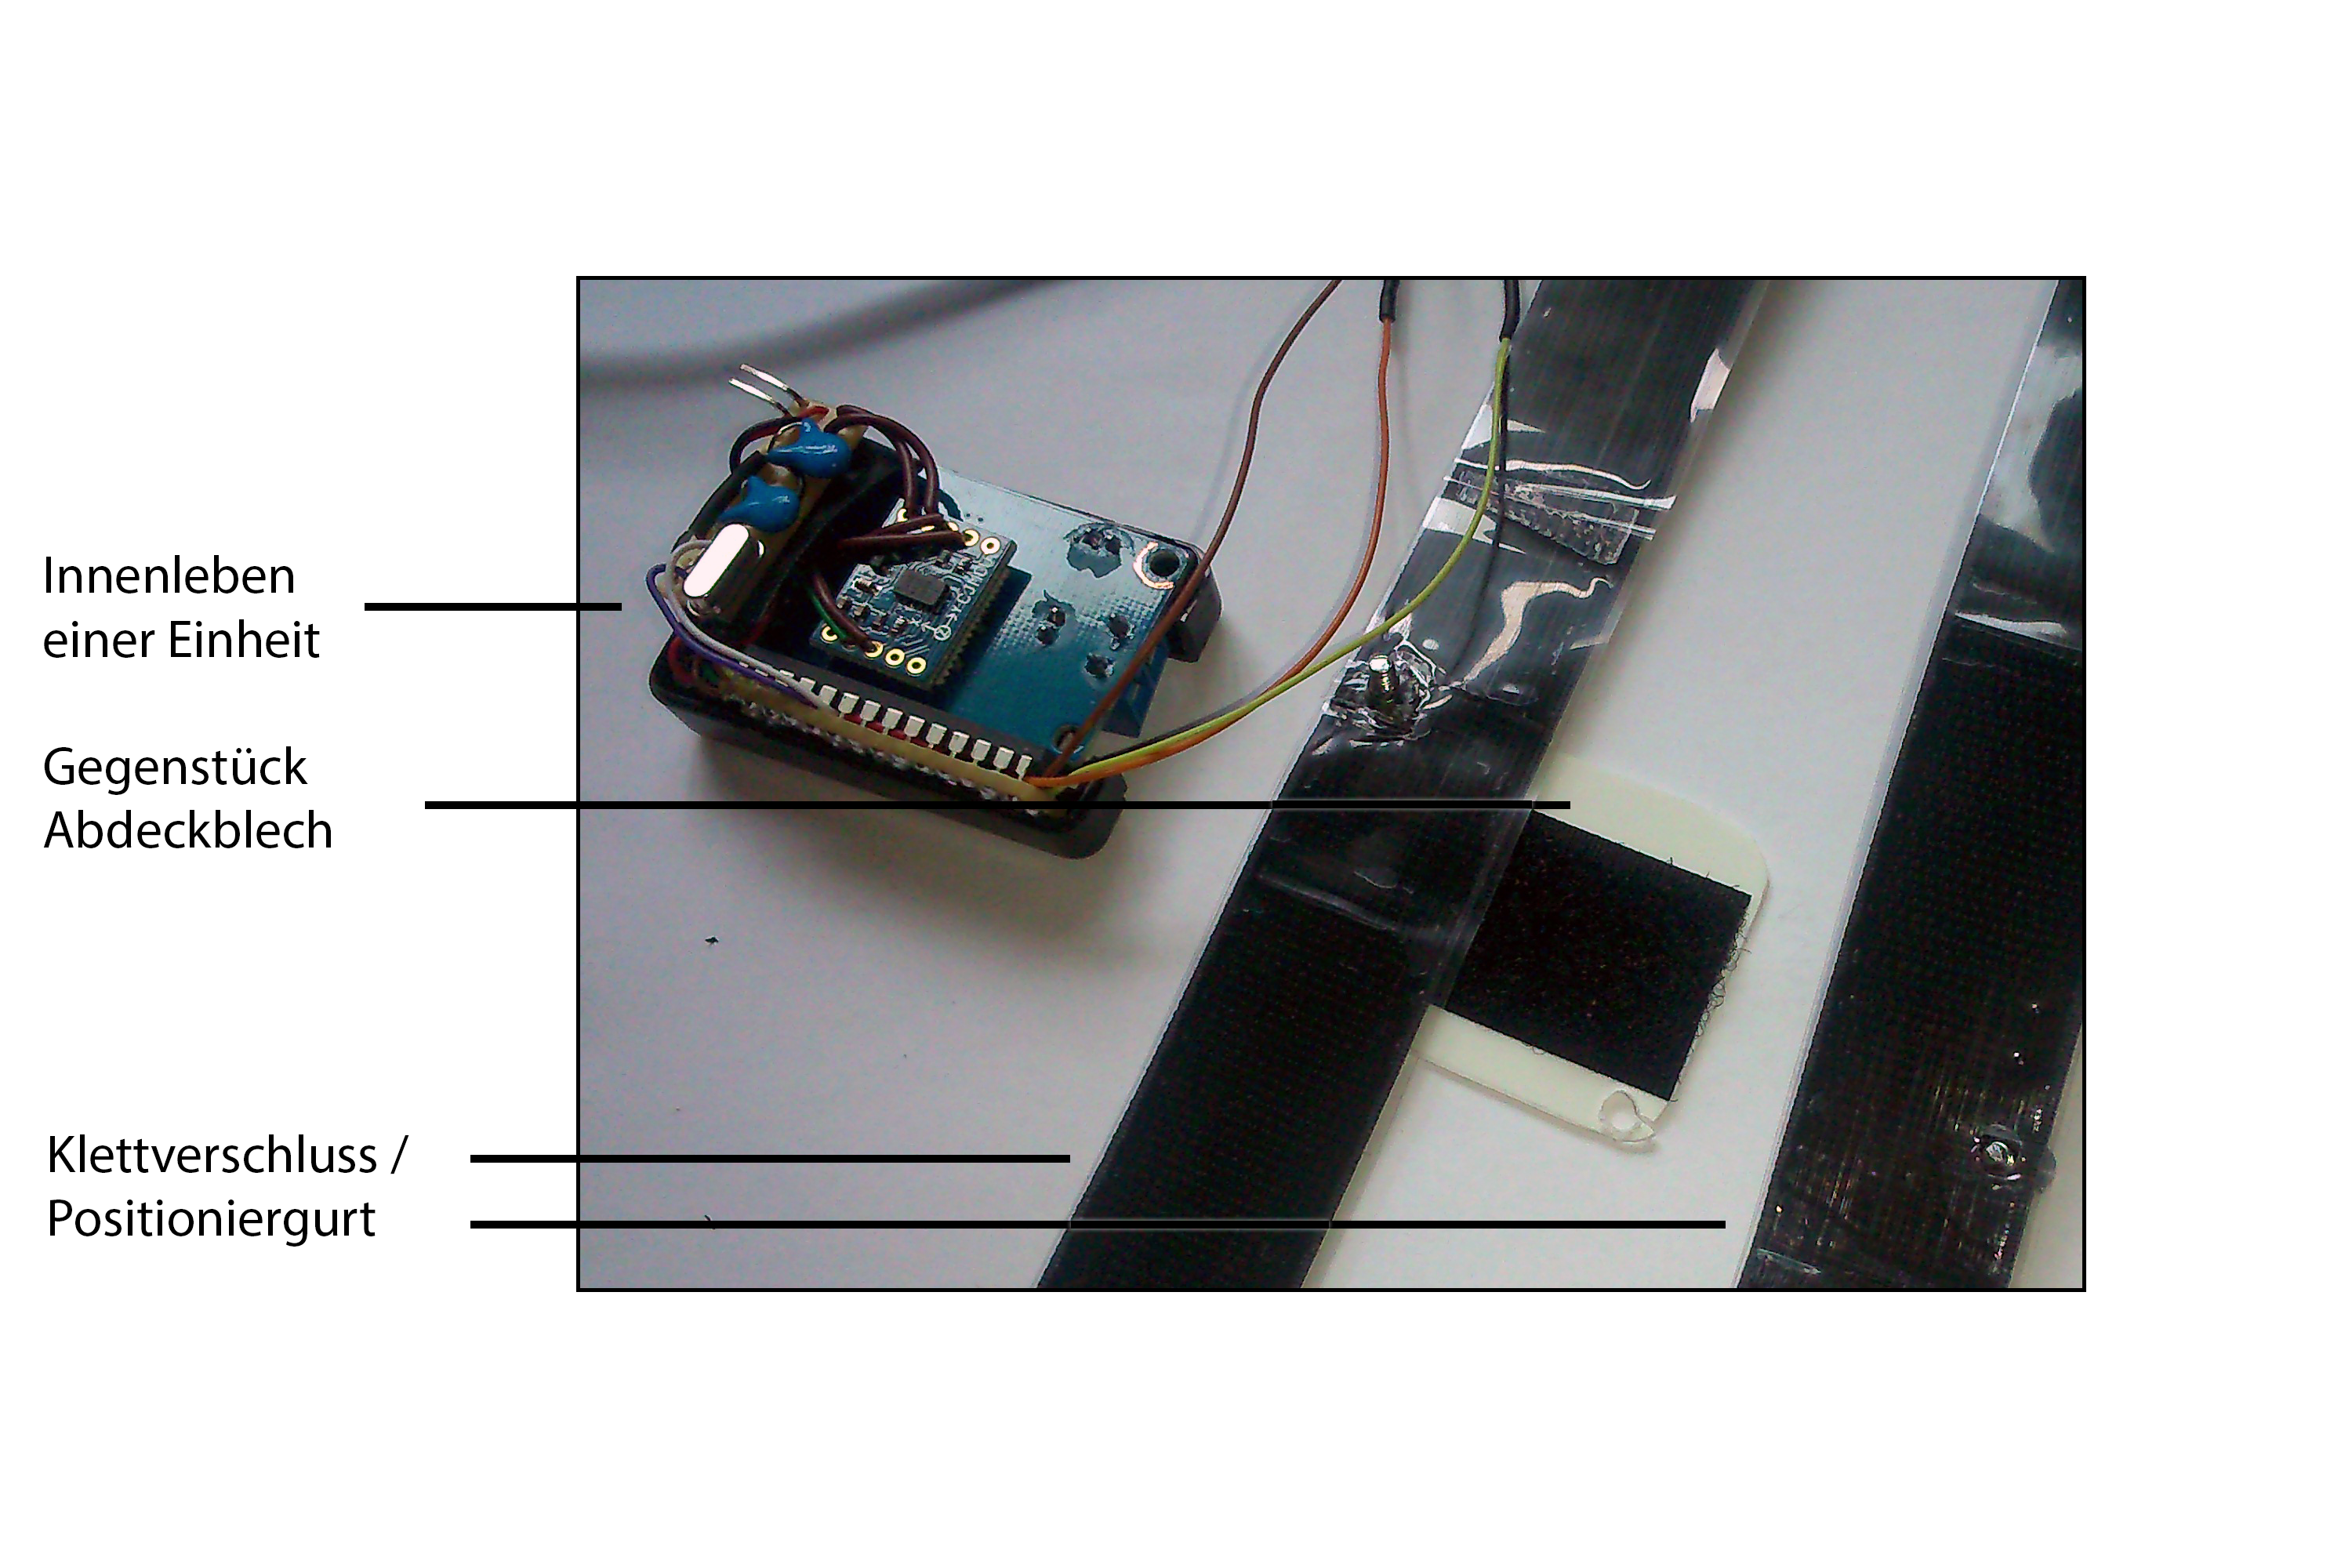
\includegraphics[width=1.0\linewidth]{Bilder/McpExecutor2515Klettverschluss}
	\caption[Betaversion einer Mcp-Executor-Einheit - Klettverschluss]{Betaversion einer Mcp-Executor-Einheit - Klettverschluss}
	\label{fig:McpExecutorBetaKlettverschluss}
\end{figure}

An dem Anzug sind ebenfalls entsprechende Gegenstücke des Klettverschlusses angebracht, sodass die Einheiten während der Bewegung nicht verrutschen. 
%
\item \textbf{Zweite Beta-Version} \\
Einige optische und wenige konstruktive Änderungen werden in der zweiten Beta-Version vorgenommen. Diese sind in Tabelle \ref{tab:McpExecutorEinheitNegAspekte2} dargestellt. 

\begin{table}[H]
	\caption{Optimierung der Beta-Version}\label{tab:McpExecutorEinheitNegAspekte2}
	\centering
	\begin{tabular}{|p{5cm}|p{5cm}|p{5cm}|}
		\hline
		\textbf{Negativer Aspekt} & \textbf{Begründung} &  \textbf{Lösung}\\
		\hline
		Leitungen Rxd, Txd, Reset liegen vor den Anschlusspins & Mögliche Beschädigung & Leitungen eine Reihe weiter unten verlöten \\
		\hline
		Gehäuse ist instabil & Durch die AUssparungen deformiert sich das Gehäuse & Steg bestehen lassen \\
		\hline
		Gehäusedeckel sitzt schief & Bohrungen u. Senkungen nicht fluchtend mit Gewindestutzen & Saubere Bohrung setzen \\
		\hline
		Abdeckblech sitzt schief & 2. Gewindestutzen wurde aufgrund des Platzes entfernt & 2. Gewindestutzen bestehen lassen \\
		\hline
	\end{tabular} 
\end{table}



\end{enumerate}

